\documentclass[10pt,        % Don't change the font size!
               a4paper,     % Don't change the paper size!
               journal,     % Journal paper format
%               draft       % Enable this parameter to get a draft version.
               ]{IEEEtran}
\makeatletter


\def\markboth#1#2{\def\leftmark{\@IEEEcompsoconly{\sffamily}\MakeUppercase{\protect#1}}%
\def\rightmark{\@IEEEcompsoconly{\sffamily}\MakeUppercase{\protect#2}}}
\makeatother

% Use this package for new German hyphenation and to set some captions to German (e.g. Abstract -> Zusammenfassung)
% \usepackage[ngerman]{babel}
% Select input file coding Latin1 or UTF8.
% See "http://en.wikipedia.org/wiki/Latin1" and "http://en.wikipedia.org/wiki/Utf8" for more information
%\usepackage[latin1]{inputenc}
\usepackage[utf8]{inputenc}

\usepackage[T1]{fontenc}
% If IEEEtran.cls has not been installed into the LaTeX system files,
% manually specify the path to it like:
% \documentclass[journal]{../sty/IEEEtran}

% *** GRAPHICS RELATED PACKAGES ***
%
\ifCLASSINFOpdf
  \usepackage[pdftex]{graphicx}
  % declare the path(s) where your graphic files are
  \graphicspath{{../pdf/}{../jpeg/}}
  % and their extensions so you won't have to specify these with every instance of \includegraphics
  \DeclareGraphicsExtensions{.pdf,.jpeg,.png}
\else
  % or other class option (dvipsone, dvipdf, if not using dvips). graphicx
  % will default to the driver specified in the system graphics.cfg if no driver is specified.
  % \usepackage[dvips]{graphicx}
  % declare the path(s) where your graphic files are
  % \graphicspath{{../eps/}}
  % and their extensions so you won't have to specify these with every instance of \includegraphics
  % \DeclareGraphicsExtensions{.eps}
\fi

% *** MATH PACKAGES ***
%
%\usepackage[cmex10]{amsmath}
% A popular package from the American Mathematical Society that provides many useful and powerful commands for dealing with mathematics. If using it, be sure to load this package with the cmex10 option to ensure that only type 1 fonts will utilized at all point sizes. Without this option, it is possible that some math symbols, particularly those within footnotes, will be rendered in bitmap form which will result in a document that can not be IEEE Xplore compliant!
% Also, note that the amsmath package sets \interdisplaylinepenalty to 10000 thus preventing page breaks from occurring within multiline equations. Use:
%\interdisplaylinepenalty=2500
% after loading amsmath to restore such page breaks as IEEEtran.cls normally does. amsmath.sty is already installed on most LaTeX systems. The latest version and documentation can be obtained at: http://www.ctan.org/tex-archive/macros/latex/required/amslatex/math/

% *** SPECIALIZED LIST PACKAGES ***
%
%\usepackage{algorithmic}
% algorithmic.sty was written by Peter Williams and Rogerio Brito.
% This package provides an algorithmic environment fo describing algorithms. You can use the algorithmic environment in-text or within a figure environment to provide for a floating algorithm. Do NOT use the algorithm floating environment provided by algorithm.sty (by the same authors) or algorithm2e.sty (by Christophe Fiorio) as IEEE does not use dedicated algorithm float types and packages that provide these will not provide correct IEEE style captions. The latest version and documentation of algorithmic.sty can be obtained at: http://www.ctan.org/tex-archive/macros/latex/contrib/algorithms/
% There is also a support site at: http://algorithms.berlios.de/index.html
% Also of interest may be the (relatively newer and more customizable) algorithmicx.sty package by Szasz Janos: http://www.ctan.org/tex-archive/macros/latex/contrib/algorithmicx/

% *** ALIGNMENT PACKAGES ***
%
%\usepackage{array}
% Frank Mittelbach's and David Carlisle's array.sty patches and improves the standard LaTeX2e array and tabular environments to provide better appearance and additional user controls. As the default LaTeX2e table generation code is lacking to the point of almost being broken with respect to the quality of the end results, all users are strongly advised to use an enhanced (at the very least that provided by array.sty) set of table tools. array.sty is already installed on most systems. The latest version and documentation can be obtained at: http://www.ctan.org/tex-archive/macros/latex/required/tools/

%\usepackage{mdwmath}
%\usepackage{mdwtab}
% Also highly recommended is Mark Wooding's extremely powerful MDW tools, especially mdwmath.sty and mdwtab.sty which are used to format equations and tables, respectively. The MDWtools set is already installed on most LaTeX systems. The lastest version and documentation is available at: http://www.ctan.org/tex-archive/macros/latex/contrib/mdwtools/

% IEEEtran contains the IEEEeqnarray family of commands that can be used to generate multiline equations as well as matrices, tables, etc., of high quality.

%\usepackage{eqparbox}
% Also of notable interest is Scott Pakin's eqparbox package for creating (automatically sized) equal width boxes - aka "natural width parboxes".
% Available at: http://www.ctan.org/tex-archive/macros/latex/contrib/eqparbox/

% *** SUBFIGURE PACKAGES ***
%\usepackage[tight,footnotesize]{subfigure}
% subfigure.sty was written by Steven Douglas Cochran. This package makes it easy to put subfigures in your figures. e.g., "Figure 1a and 1b". For IEEE work, it is a good idea to load it with the tight package option to reduce the amount of white space around the subfigures. subfigure.sty is already installed on most LaTeX systems. The latest version and documentation can be obtained at: http://www.ctan.org/tex-archive/obsolete/macros/latex/contrib/subfigure/
% subfigure.sty has been superceeded by subfig.sty.

%\usepackage[caption=false]{caption}
%\usepackage[font=footnotesize]{subfig}
% subfig.sty, also written by Steven Douglas Cochran, is the modern replacement for subfigure.sty. However, subfig.sty requires and automatically loads Axel Sommerfeldt's caption.sty which will override IEEEtran.cls handling of captions and this will result in nonIEEE style figure/table captions. To prevent this problem, be sure and preload caption.sty with its "caption=false" package option. This is will preserve IEEEtran.cls handing of captions. Version 1.3 (2005/06/28) and later  (recommended due to many improvements over 1.2) of subfig.sty supports the caption=false option directly:
%\usepackage[caption=false,font=footnotesize]{subfig}
% The latest version and documentation can be obtained at: http://www.ctan.org/tex-archive/macros/latex/contrib/subfig/
% The latest version and documentation of caption.sty can be obtained at: http://www.ctan.org/tex-archive/macros/latex/contrib/caption/

% *** FLOAT PACKAGES ***
%
%\usepackage{fixltx2e}
% fixltx2e, the successor to the earlier fix2col.sty, was written by Frank Mittelbach and David Carlisle. This package corrects a few problems in the LaTeX2e kernel, the most notable of which is that in current LaTeX2e releases, the ordering of single and double column floats is not guaranteed to be preserved. Thus, an unpatched LaTeX2e can allow a single column figure to be placed prior to an earlier double column figure. The latest version and documentation can be found at:
% http://www.ctan.org/tex-archive/macros/latex/base/

%\usepackage{stfloats}
% stfloats.sty was written by Sigitas Tolusis. This package gives LaTeX2e the ability to do double column floats at the bottom of the page as well as the top. (e.g., "\begin{figure*}[!b]" is not normally possible in LaTeX2e). It also provides a command:
%\fnbelowfloat
% to enable the placement of footnotes below bottom floats (the standard LaTeX2e kernel puts them above bottom floats). This is an invasive package which rewrites many portions of the LaTeX2e float routines. It may not work with other packages that modify the LaTeX2e float routines. The latest version and documentation can be obtained at: http://www.ctan.org/tex-archive/macros/latex/contrib/sttools/
% Documentation is contained in the stfloats.sty comments as well as in the presfull.pdf file. Do not use the stfloats baselinefloat ability as IEEE does not allow \baselineskip to stretch. Authors submitting work to the IEEE should note that IEEE rarely uses double column equations and that authors should try to avoid such use. Do not be tempted to use the cuted.sty or midfloat.sty packages (also by Sigitas Tolusis) as IEEE does not format its papers in such ways.

%\ifCLASSOPTIONcaptionsoff
%  \usepackage[nomarkers]{endfloat}
% \let\MYoriglatexcaption\caption
% \renewcommand{\caption}[2][\relax]{\MYoriglatexcaption[#2]{#2}}
%\fi
% endfloat.sty was written by James Darrell McCauley and Jeff Goldberg. This package may be useful when used in conjunction with IEEEtran.cls' captionsoff option. Some IEEE journals/societies require that submissions have lists of figures/tables at the end of the paper and that figures/tables without any captions are placed on a page by themselves at the end of the document. If needed, the draftcls IEEEtran class option or \CLASSINPUTbaselinestretch interface can be used to increase the line spacing as well. Be sure and use the nomarkers option of endfloat to prevent endfloat from "marking" where the figures would have been placed in the text. The two hack lines of code above are a slight modification of that suggested by in the endfloat docs (section 8.3.1) to ensure that the full captions always appear in the list of figures/tables - even if the user used the short optional argument of \caption[]{}.
% IEEE papers do not typically make use of \caption[]'s optional argument, so this should not be an issue. A similar trick can be used to disable captions of packages such as subfig.sty that lack options to turn off the subcaptions:
% For subfig.sty:
% \let\MYorigsubfloat\subfloat
% \renewcommand{\subfloat}[2][\relax]{\MYorigsubfloat[]{#2}}
% For subfigure.sty:
% \let\MYorigsubfigure\subfigure
% \renewcommand{\subfigure}[2][\relax]{\MYorigsubfigure[]{#2}}
% However, the above trick will not work if both optional arguments of the \subfloat/subfig command are used. Furthermore, there needs to be a description of each subfigure *somewhere* and endfloat does not add subfigure captions to its list of figures. Thus, the best approach is to avoid the use of subfigure captions (many IEEE journals avoid them anyway) and instead reference/explain all the subfigures within the main caption. The latest version of endfloat.sty and its documentation can obtained at: http://www.ctan.org/tex-archive/macros/latex/contrib/endfloat/
% The IEEEtran \ifCLASSOPTIONcaptionsoff conditional can also be used later in the document, say, to conditionally put the References on a  page by themselves.

% correct bad hyphenation here
\hyphenation{op-tical net-works semi-conduc-tor}

\begin{document}
\title{Relational and NoSQL Databases: A Comparison and Introduction to Hybrid and Mining Frameworks}

% author names and IEEE memberships note positions of commas and nonbreaking spaces ( ~ ) LaTeX will not break a structure at a ~ so this keeps an author's name from being broken across two lines.
% use \thanks{} to gain access to the first footnote area a separate \thanks must be used for each paragraph as LaTeX2e's \thanks was not built to handle multiple paragraphs.

\author{Teodor Fratiloiu}% <-this % stops a space
%\thanks{M. Shell is with the Department
%of Electrical and Computer Engineering, Georgia Institute of Technology, Atlanta,
%GA, 30332 USA e-mail: (see http://www.michaelshell.org/contact.html).}% <-this % stops a space
%\thanks{J. Doe and J. Doe are with Anonymous University.}% <-this % stops a space
%\thanks{Manuscript received April 19, 2005; revised January 11, 2007.}}

% note the % following the last \IEEEmembership and also \thanks - 
% these prevent an unwanted space from occurring between the last author name
% and the end of the author line. i.e., if you had this:
% 
% \author{....lastname \thanks{...} \thanks{...} }
%                     ^------------^------------^----Do not want these spaces!
%
% a space would be appended to the last name and could cause every name on that
% line to be shifted left slightly. This is one of those "LaTeX things". For
% instance, "\textbf{A} \textbf{B}" will typeset as "A B" not "AB". To get
% "AB" then you have to do: "\textbf{A}\textbf{B}"
% \thanks is no different in this regard, so shield the last } of each \thanks
% that ends a line with a % and do not let a space in before the next \thanks.
% Spaces after \IEEEmembership other than the last one are OK (and needed) as you are supposed to have spaces between the names. For what it is worth, this is a minor point as most people would not even notice if the said evil space somehow managed to creep in.

% The paper headers
\markboth{Scientific Seminar on Security in Information Technology, Winter Semester 2020/2021}%
{Teodor Fratiloiu: Comparison of SQL Relational Databases and NoSQL Graph Databases}

%\markboth{Journal of \LaTeX\ Class Files,~Vol.~6, No.~1, January~2007}%
%{Shell \MakeLowercase{\textit{et al.}}: Bare Demo of IEEEtran.cls for Journals}
% The only time the second header will appear is for the odd numbered pages
% after the title page when using the twoside option.
% 
% *** Note that you probably will NOT want to include the author's ***
% *** name in the headers of peer review papers.                   ***
% You can use \ifCLASSOPTIONpeerreview for conditional compilation here if you desire.

% If you want to put a publisher's ID mark on the page you can do it like this:
%\IEEEpubid{0000--0000/00\$00.00~\copyright~2007 IEEE}
% Remember, if you use this you must call \IEEEpubidadjcol in the second column for its text to clear the IEEEpubid mark.

%\IEEEspecialpapernotice{(Invited Paper)} % use for special paper notices
\maketitle


\begin{abstract}
%\boldmath
Classic, relational, SQL databases have proven their reliability, and versatility, in many different scenarios over the past few decades. However wide their field of application may be though, there are still many situations, where one can be limited by the constraints of these traditional data structures. Efficiently querying very large user databases is one such situation. In this work, we are going to investigate a different paradigm for  big data management: Graph Databases. This relatively new breed of data management systems are already finding wide acceptance, and are being actively deployed, across many industries. Use cases such as social media applications come to mind, where scalability is of prime importance since datasets could theoretically achieve infinite dimensions. In this work, we will compare Graph (NoSQL) databases, as well as their strengths, and weaknesses, to classic, relational SQL databases. We will also dive into innovative new technologies, which promise to enable completely new ways of working with databases and making sense of the data inside.
\end{abstract}

\textbf{Keywords:} Relational Database, NoSQL Graph Database, Tablespace, Graph Mining, Hybrid (No)SQL 
% IEEEtran.cls defaults to using nonbold math in the Abstract.
% This preserves the distinction between vectors and scalars. However, if the journal you are submitting to favors bold math in the abstract, then you can use LaTeX's standard command \boldmath at the very start of the abstract to achieve this. Many IEEE journals frown on math in the abstract anyway.

% Note that keywords are not normally used for peerreview papers.
%\begin{IEEEkeywords}
%IEEEtran, journal, \LaTeX, paper, template.
%\end{IEEEkeywords}

% For peer review papers, you can put extra information on the cover page as needed:
% \ifCLASSOPTIONpeerreview
% \begin{center} \bfseries EDICS Category: 3-BBND \end{center}
% \fi
% For peerreview papers, this IEEEtran command inserts a page break and creates the second title. It will be ignored for other modes.
% \IEEEpeerreviewmaketitle


\section{Introduction}
Databases have been used as the prime way of storing data in digital formats for the better part of the past 70 years since computer memory became large enough to enable this in the 1960s. It is safe to assume that virtually every kind of tabular data, which has since been digitalized, has been converted into one such database, or a closely related approximation thereof. \cite{bachman_1973} \par
The history of databases has often been divided into 3 separate phases: firstly, there was the \textit{classical} period of navigational databases (which strongly relied on the period's ever present memory pointers). This was followed by the invention of the relational (SQL) database by IBM's researchers in the early 1970s \cite{codd_1970}. Lastly, around the turn of the millennia, researchers came up with the modern, post-SQL (or NoSQL) database, which has the distinction of having \textit{no fixed structure}, or much in the way of theoretical constraints related to its overall architecture, if at all. \par
The reason for the existence of these new, very flexible types of databases has much to do with the main issue of classic, SQL databases. It is the exponential way in which hardware requirements scale up with the amount of data stored. This means that it becomes exponentially more challenging to maintain speed, RAM, and storage amounts within reasonable constraints as the amount of stored data increases. This problem of SQL databases has been steadily developing over the decades, and it has to do with the difficulties that arise when mixing legacy database rules with the realities of modern, distributed, and connected devices. \cite{IEEEpaper1:comparison} \par
Let us, therefore, introduce NoSQL databases. The main difference between these, and SQL databases, is how they scale. While SQL databases scale \textit{vertically}, NoSQL databases scale \textit{horizontally}. Specifically, it is the BASE (Basically Available State and Eventually Consistent) property of NoSQL databases which enables them to be a perfect choice for very large, connected, amounts of data. \par
For this paper, we shall consider the term \textit{relational} database (RDBMS) as synonymous to \textit{SQL} database, and the term \textit{NoSQL} database as equivalent to \textit{Graph} database, unless other specified. As such, the respective pairs of terms will be used interchangeably. \par
It has been proved in the research literature, as well as by the industry, that Graph databases perform radically better than relational databases for big data applications. \cite{IEEEpaper1:comparison} This is especially true in scenarios where one can use the connected nature of data to their advantage. One prominent example of this is how Neo4j (NoSQL) performs much better than Oracle 11g (SQL). \cite{comparison_2015} \par
However, let us not forget that Graph databases are not the only kind of NoSQL database out there. There are four types in total. Let us examine these in detail.
\subsection{Types of NoSQL Databases}
There are four different kinds of NoSQL databases. Their properties and use scenarios depend on the needs and requirements of the applications in which they are used. 
\begin{itemize}
	\item \textbf{Key-Value}: these are, essentially, hash tables, where unique hash keys are used to search for and point to specific values; the contents themselves are not used during queries.
	\item \textbf{Document}: Data is stored as a key/value tuple, and both the content, as well as the \textit{key} are used for searches, which constitutes a major difference from the type above. Documents of this type can be stored in XML, JSON, and BSON formats, and popular apps using this type of database include MongoDB and CouchDB.
	\item \textbf{Wide-Column}: These databases are made unique by the hybrid approach used to store data. In this scenario, which is mainly used in \textit{cluster environments} and for distributed data, we will combine the features of relational databases with a key-value storage schema. Examples such as Hbase, Cassandra, and Accumulo spring to mind.
	\item \textbf{Graph}: This type is used where the data has a high degree of connectivity since such databases can naturally store relationships between Independent pieces of data. Examples include Neo4j, Pregel, ArrangoDB, and OrientDB. 
\end{itemize}
Actual examples, together with actual package names, query languages and properties, can be found in \textit{Table \ref{table_types_nosql}}. \cite{IEEEpaper1:comparison}

\begin{table}[!t]
	\renewcommand{\arraystretch}{1.3} % increase table row spacing, adjust to taste
	\caption{Types of NoSQL Databases with Examples}
	\label{table_types_nosql}
	\centering
	\begin{tabular}{|c|c|c|c|}
		\hline
		Type & Package & Query Language & Property Support  \\
		\hline
		Graph & Neo4j & CypherQL & ACID \\
		\hline
		Graph & ArangoDB & AQL & \\
		\hline
		 & Hive & HQL & \\
		\hline
		Graph & OrientDB & SQL & ACID \\
		\hline
		Key-Value & Riak & &  \\
		\hline
		Key-Value & Redis & & \\
		\hline
		Key-Value & Voldemort & & \\
		\hline
		Column & Hbase & & \\
		\hline
		Column & Accumulo & & \\
		\hline
		Document & MongoDB & & \\
		\hline
		Document & CouchDB & & \\
		\hline
	\end{tabular}
\end{table}

Having now delivered our remarks about the fundamental differences between SQL and Graph Databases, and the different types there are out there, let us proceed with a more detailed description of the current state of development in the industry.

\section{State of the Art}
In this section, we shall look into, and compare, the different properties of SQL and NoSQL databases. For starters, let us revisit the scalability issue. As previously discussed, the more varied and larger the amount of data present in a SQL database, the more CPU and RAM a system will need. This is because relational databases scale \textit{vertically}, in contrast to NoSQL databases, which scale \textit{horizontally}. \par
SQL databases are traditionally a good fit for applications where data integrity and security are important, since cryptographic procedures and information security can be more easily implemented in such a scenario. NoSQL databases, however, are a great fit for very large, and growing, datasets, because they allow us to, for instance, add extra storage servers to an existing system with minimal intervention. The following theoretical exercise might help one understand this better. \par
\subsection{The CAP Theorem}
To enable us to better understand the fundamental differences between relational and Graph databases, let us introduce Eric Brewer's \textit{CAP Theorem} - Consistency, Availability and Partition Tolerance. \cite{brewer_cap_theorem} A term by term analysis looks as follows: \textit{Consistency} describes the property of a system of achieving a \textit{stable state}, after one (or more) \textit{write} operations. \textit{Availability} describes data, namely, it being present and ready for \textit{read} operations at one desired spot, after having been modified (right there or somewhere else). \textit{Partition Tolerance} refers to a system's ability to continue functioning, even if its resources are spread over different locations and nodes. \par
In relational databases, primary keys are used to ensure that data is \textit{unique} - it exists in one single location. NoSQL databases, on the other hand, and in no small part due to their distributed nature, cannot provide such a feature. But let us not believe that this would have to be a bad thing. NoSQL databases will, because of this, be much more flexible and responsive to the changes one would experience in a connected system, for instance. Moreover, tracking interaction between different objects is much easier in this scenario. \par
However, we shall quickly realize that there is one obvious \textit{catch} to all of this: a distributed database system can never offer true CAP features. Not in a logically rigorous manner, at least. That is because the intrinsic nature of how the data is stored in such a system cannot guarantee total and immediate consistency. Let us think about how data propagates across the internet. For the purpose of this, let one imagine they would change one's online profile picture for their Google profile, on their desktop. After the change is done, let one immeaditely pick up their smartphone and open the YouTube app, where they had already been logged in with their Google account. One can very sensibly assume that the picture the user would see on their smartphone, at least for the first few moments, will be their old profile picture. This goes to prove that, for a brief period of time, that one user had \textit{two different profile pictures}, at the same time. A state which very obviously contradicts any form of consistency. \par
To sum up, let one remember that relational databases traditionally possess all 3 CAP properties, whereas NoSQL databases (depending on the implementation) customarily only support the \textit{Availability} and \textit{Partition Tolerance} parts, but lack the \textit{Consistency} feature. Let us now look out over on the other side of the fence, and see how relational, SQL databases fare. \par
As such, let us now dive into the specific advantages and disadvantages afforded by the underlying technologies and the very nature of these two kinds of databases, respectively. 

\section{Methods and Contributions}
\subsection{On SQL and the Importance of Information Security}

As previously discussed, relational databases support the ACID (atomicity, consistency, isolation, and durability) property. This ensures that we can reliably implement data security-related measures for our data. For instance, financial applications need to provide guarantees that money sums are accurate all the time, and that there is absolutely no ambiguity whatsoever about how much one's account is worth at one specific time-point. As a comparison, let us draw once again upon the example of changing one's profile picture and waiting for it to propagate across different devices. This would be unacceptable for a financial application since it could potentially allow for tampering and abuse. Let one imagine a very trading fast bot that would capitalize on such a loophole by performing 2 identical purchase orders in very fast succession, faster than the system could account for the cost of the first one, and therefore buy the second asset for virtually zero money since their total capital had remained unchanged since the first buy. \par
For this reason, we are limited to only using SQL databases for such sensitive applications as financial platforms. Using them requires us to separate and log our different actions utilizing \textit{orders} or \textit{transactions} - which ensures atomicity and isolation. Each of these transactions would then need to be centrally approved before changing any data in the actual database - therefore ensuring consistency and durability. Unfortunately, such guarantees would never be possible with a pure Graph database (one without modifications and extra provisions, that is). As such, let us look into how we could potentially get the benefits of both worlds, with a hybrid approach.\par

\subsection{The Hybrid Approach}
In their 2019 paper, Vyawahare and Karde \cite{IEEEpaper3:hybrid} make a comprehensive review of past scientific literature on the topic of hybrid databases. Let us explain their main points, as well as their contributions. \par
The main assumption the authors make about enabling a hybrid database approach is the fact that we need a minimum of 2 databases, of the same or different kinds, which we can access through a common \textit{abstraction layer}. In layman's terms, this implies that one would have to come up with a know-it-all software framework, capable of linking databases of all kinds, and enabling a coherent mix-match of data types of all shapes and sizes, which would ideally work together. \par
The workflow proposed in the paper is relatively straightforward. One would start by loading and analyzing data, determining whether its structure would be a better fit for either the relational or the NoSQL sides of the harmonized, hybrid database, then store that data appropriately. Obviously, there are many variations that can be made to these steps. For example, one could use the hybrid framework to simply convert databases of one type into the other, to benefit from the advantages of the other side. One could also use the framework to harmonize the types of queries used in their apps and reduce the overhead generated by having to use multiple querying languages. Finally, the authors go into some detail about the advantages of keeping data \textit{in memory}. These mostly revolve around access times, and availability, plus reducing the storage and processing overhead generated by real-time data conversion. \par
Having now seen the hybrid approach to database design, let us look into how we can make sense of the data inside our databases by what is known as \textit{Graph Mining Framework}, as described in \cite{IEEEpaper2:mining}.

\subsection{Data Mining and Graph Visualization}
In the day and age of the internet, where data is being generated and saved at \textit{breakneck} speed, making sense of this content has become a matter of automated analysis. Conveniently, one very important application of Graph Databases is their enabling more robust, and faster, data mining. \par
The main features one \textit{graph mining} tool would have to provide include graph preprocessing, association discovery, cluster detection, and graph visualization. Let us investigate these in detail. \par
Firstly, graph preprocessing is to be understood as an \textit{umbrella} term for all the necessary steps to transform data from an arbitrary format, such as \textit{XML} or the result of web-crawling, into a specific format for our application. The data would be stored as an undirected graph, with non-unique labeled edges. \cite{IEEEpaper2:mining} Secondly, when it comes to association discovery, we could set arbitrary thresholds for the number of edges connecting different nodes and the types of nodes we are looking at. This would allow us to, for example, discover popular actor-director pairs in a movie database. Third, if we were to detect data clusters, we could, for instance, use algorithms such as trawling \cite{paper_2_ref_1}, shingling \cite{paper_2_ref_2}, connection subgraphs \cite{paper_2_ref_3}, or maximum clique detection \cite{paper_2_ref_4}, which would enable our framework to answer questions such as identifying one user's social media friends, or the number of news articles on one particular topic. Lastly, a form of graph visualization would allow one to input data in some arbitrary text-based descriptive format and receive a visual representation of this graph. \par
One such framework would enable data scientists to make more sense of the plethora of data available in different places. 

\section{Results} 
For this section, we will compare the access (read and write) performance of different types of databases. 
\subsection{Numerical Comparisons}
For this subsection, let us observe some plots. In \textit{Figure \ref{graph_phys_vs_neo4j}}, we can see how a physically optimized relational database fares against a graph database. \textit{Figure \ref{graph_no_phys_vs_neo4j}} shows us the longer access times when there is no physical optimization. The actual numerical times are presented in \textit{Figure \ref{table_phys_vs_neo4j}}, and \textit{Figure \ref{table_no_phys_vs_neo4j}}, respectively. \par
\begin{figure}[!t]
	\centering
	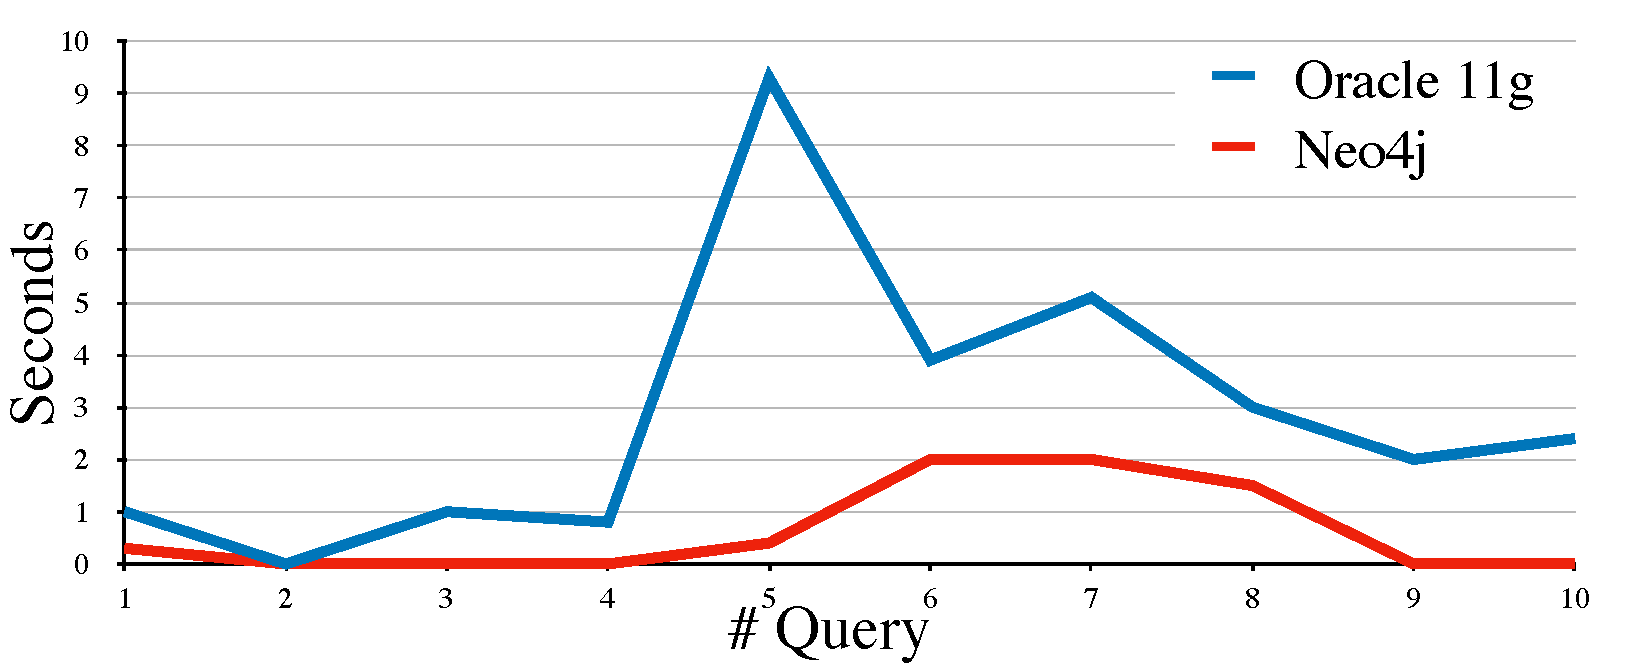
\includegraphics[width=2.5in]{plots/phys_vs_neo4j}
	\caption{Performance Comparison of Neo4j with a RDBS with physical tuning \cite{IEEEpaper1:comparison}}
	\label{graph_phys_vs_neo4j}
\end{figure}

\begin{figure}[!t]
	\centering
	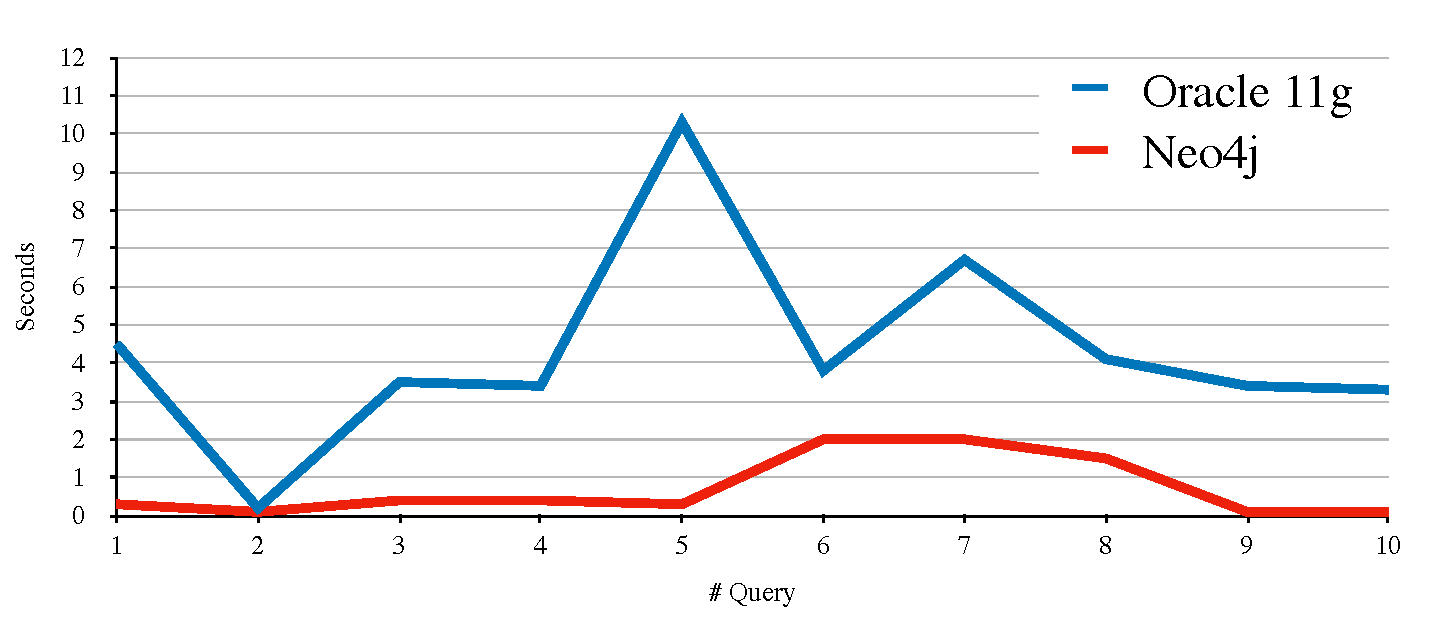
\includegraphics[width=2.5in]{plots/no phys vs neo4j}
	\caption{Performance Comparison of Neo4j with a RDBS with no physical tuning \cite{IEEEpaper1:comparison}}
	\label{graph_no_phys_vs_neo4j}
\end{figure}

\begin{figure}[!t]
	\centering
	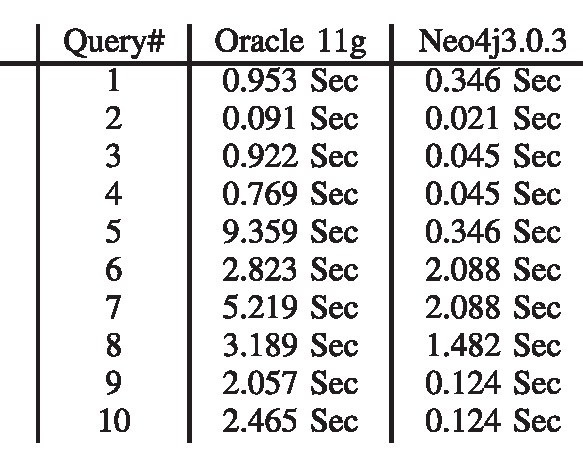
\includegraphics[width=2.5in]{plots/phys vs neo4j table}
	\caption{Performance Comparison of (physically optimized) Oracle 11g with Neo4j \cite{IEEEpaper1:comparison}}
	\label{table_phys_vs_neo4j}
\end{figure}

\begin{figure}[!t]
	\centering
	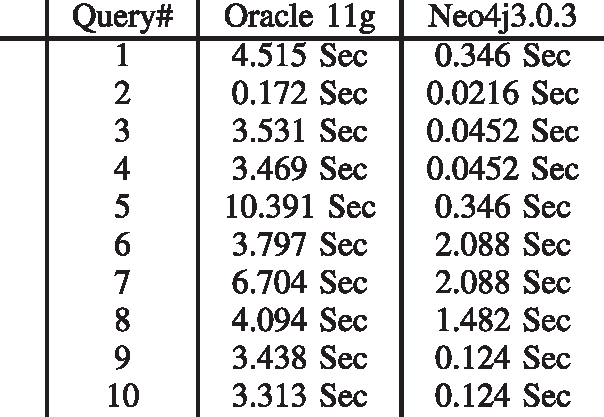
\includegraphics[width=2.5in]{plots/no tuning table}
	\caption{Performance Comparison of Oracle 11g (no physical optimization) with Neo4j \cite{IEEEpaper1:comparison}}
	\label{table_no_phys_vs_neo4j}
\end{figure}

\subsection{Relational Database Design Optimization}
In this subsection, we shall examine the results and performance achieved by tuning relational databases, why this is so important, and why one should always consider doing it, both when deploying a product, and when running benchmarks on standard data to determine speed. \par
Let us look into how the performance of classic databases can be optimized. To this end, a process called \textit{tuning} can be involved. For instance, to improve the query performance of \textit{Oracle 11g} tables, we can use different tablespaces for each individual schema.  This results in more than one data file used for storage, which in turn allows us to optimize the size of the memory blocks used. This is useful, since both small and large memory block sizes can be desirable, depending on the scenario. For example, \textit{warehouse-type} data requires large memory blocks, whereas, for \textit{OLTP} type data, we are required to use small block sizes. The total space allocation in a file is defined as an \textit{extent}, whereas one unit of I/O data is referred to as a \textit{block}. 
The ACID (Atomicity, Consistency Isolation, Durability) property of SQL databases helps maintain consistency across the data and enables efficient polling and querying, but even this is eventually overcome by the sheer size of modern databases for online, user-generated content. \par
Even if SQL databases store data in separate tables, and normalization techniques, such as 1NF, 2NF, and 3NF, can be used to reduce redundancy, this method remains unsuitable for modern applications. For instance, although it is possible to \textit{join} queries when searching a SQL database for entries, this too becomes inefficient when using 20 or more parameters. \par
Judging by this, and by the thoughts expressed in the previous subsection, we can conclude that both sides prove to have specific design limitations, which are impossible to directly overcome. \par
\subsection{Main Take-Aways}
Firstly, it is widely accepted that NoSQL, Graph databases are the desirable way to store data  when systems are distributed and when flexibility, and redundancy, are needed. Such fields as online shops, social media, or some remote working tools rely on this type of system architecture, to ensure responsiveness and reliable operation for multi-user collaboration. Further development and standardization of such systems could potentially open the doors to increased efficiency and reduced costs across the industry. \par
On the other hand, relational databases still play a very important role in centralized, high-value, or mission-critical data. It is only with this type of database that one can ensure the reliable storage of such information like medical records, employment and financial histories, or voter registrations. Future research in this area could involve the development of even more sophisticated file systems, optimized for fast flash storage, or increasing information security by means of tightening standards for advanced encryption and by rolling out more and more granular access control. \par 
Moreover, let us once more stress the fact that we do not assert the superiority of either database type over the other. We remain strongly convinced that both have their own strengths and weaknesses, which one only needs to be aware of when making the choice about which best suits their needs. It is exactly for this reason that we presented the Hybrid approach to database design, in which many see an acceptable compromise. \par

\section{Conclusion}
Having now accomplished what we set out to do - namely to present a thorough analysis, and comparison, of the two most common types of databases in use throughout industries in this day and age, let us now deliver the closing remarks and express our hope that have at least awoken the community's interest for further research on the topic. 

% if have a single appendix:
%\appendix[Proof of the Zonklar Equations]
% or
%\appendix  % for no appendix heading
% do not use \section anymore after \appendix, only \section*
% is possibly needed

% use appendices with more than one appendix then use \section to start each appendix. You must declare a \section before using any \subsection or using \label (\appendices by itself starts a section numbered zero.)

% \appendices
% \section{Proof of the First Zonklar Equation}
% Appendix one text goes here.

% you can choose not to have a title for an appendix if you want by leaving the argument blank
% \section{}
% Appendix two text goes here.

% use section* for acknowledgement
%\section*{Acknowledgment}
%The authors would like to thank...


% Can use something like this to put references on a page by themselves when using endfloat and the captionsoff option.
\ifCLASSOPTIONcaptionsoff
  \newpage
\fi



% trigger a \newpage just before the given reference number - used to balance the columns on the last page adjust value as needed - may need to be readjusted if the document is modified later
%\IEEEtriggeratref{8}
% The "triggered" command can be changed if desired:
%\IEEEtriggercmd{\enlargethispage{-5in}}

% references section

% can use a bibliography generated by BibTeX as a .bbl file
% BibTeX documentation can be easily obtained at: http://www.ctan.org/tex-archive/biblio/bibtex/contrib/doc/
% The IEEEtran BibTeX style support page is at: http://www.michaelshell.org/tex/ieeetran/bibtex/
%\bibliographystyle{IEEEtran} % argument is your BibTeX string definitions and bibliography database(s)
%\bibliography{IEEEabrv,../bib/paper}
%
% <OR> manually copy in the resultant .bbl file
% set second argument of \begin to the number of references
% (used to reserve space for the reference number labels box)
\begin{thebibliography}{3}

% \bibitem{IEEEhowto:kopka}
% H.~Kopka and P.~W. Daly, \emph{A Guide to \LaTeX}, 3rd~ed.\hskip 1em plus
%   0.5em minus 0.4em\relax Harlow, England: Addison-Wesley, 1999.

\bibitem{IEEEpaper1:comparison}
Wisal Khan, Waqas Ahmad, Bin Luo and Ejaz Ahmed, SQL Database with physical database tuning technique and NoSQL graph database comparisons
(2019)

\bibitem{IEEEpaper2:mining}
Swapnil Shrivastava and Supriya N. Pal, Graph Mining Frameworks for Finding and Visualizing Substructures using Graph Databases
(2009)

\bibitem{IEEEpaper3:hybrid}
H.R. Vyawahare, P.P. Karde and V.M. Thakare, A Hybrid Database Approach Using Graph and Relational Database
(2019)

\bibitem{bachman_1973}
Bachman, Charles W., The Programmer as Navigator. Communications of the ACM. 16 (11): 653–658. doi:10.1145/355611.362534.
(1973)

\bibitem{codd_1970}
Codd, Edgar Frank, A Relational Model of Data for Large Shared Data Banks. Communications of the ACM. 13 (6): 377–387. doi:10.1145/362384.362685. S2CID 207549016
(June 1970)

\bibitem{comparison_2015}
Oussous, A., F.-Z. Benjelloun, A. A. Lahcen, and S. Belfkih, Comparison and Classication of NoSQL Databases for Big Data (in Proceedings of International Conference on Big Data, Cloud and Applications)
(2015)

\bibitem{brewer_cap_theorem}
Seth Gilbert and Nancy Lynch, "Brewer's conjecture and the feasibility of consistent, available, partition-tolerant web services", ACM SIGACT News, Volume 33 Issue 2 (2002), pg. 51–59. doi:10.1145/564585.564601.

\bibitem{paper_2_ref_1}
R. Kumar, P. Rafhavan, S. Rajagopalan, A. Tomkins, "Thrawling the Web for Emerging Cybercommunities" 1999

\bibitem{paper_2_ref_2}
D. Gibson, R. Kumar, A. Tomkins, "Extracting Large, Dense Subgraphs in Massive Graphs" 2005

\bibitem{paper_2_ref_3}
C. Faloutsos, K. McCurley, A. Tomkins, "Fast Discovery of Connection Subgraphs" 2004

\bibitem{paper_2_ref_4}
I.M. Bomze, M. Budinich, P.M. Pardalos, M. Pelillo, "The Maximum Clique Problem" 1999

\end{thebibliography}

% biography section
% 
% If you have an EPS/PDF photo (graphicx package needed) extra braces are
% needed around the contents of the optional argument to biography to prevent
% the LaTeX parser from getting confused when it sees the complicated
% \includegraphics command within an optional argument. (You could create
% your own custom macro containing the \includegraphics command to make things
% simpler here.)
%\begin{biography}[{\includegraphics[width=1in,height=1.25in,clip,keepaspectratio]{mshell}}]{Michael Shell}
% or if you just want to reserve a space for a photo:

%\begin{IEEEbiography}{Michael Shell}
%Biography text here.
%\end{IEEEbiography}

% if you will not have a photo at all:
%\begin{IEEEbiographynophoto}{John Doe}
%Biography text here.
%\end{IEEEbiographynophoto}

% insert where needed to balance the two columns on the last page with
% biographies
%\newpage

%\begin{IEEEbiographynophoto}{Jane Doe}
%Biography text here.
%\end{IEEEbiographynophoto}

% You can push biographies down or up by placing a \vfill before or after them. The appropriate use of \vfill depends on what kind of text is on the last page and whether or not the columns are being equalized.

%\vfill

% Can be used to pull up biographies so that the bottom of the last one is flush with the other column.
%\enlargethispage{-5in}

\end{document}


